
\documentclass[11pt]{article}

\usepackage[margin=1in]{geometry}
\usepackage{amsmath,amssymb}
\usepackage{graphicx}
\usepackage{booktabs}
\usepackage{natbib}
\usepackage[hidelinks]{hyperref}
\usepackage{microtype}

\title{Memory-Weighted Selection: Middleware for Continuity and Governed Behaviour in LLM Systems}
\author{Marcos Verrell\\Independent Researcher}
\date{}

\begin{document}
\maketitle

\begin{abstract}
Large language model systems often rely on direct base-model emission or retrieval-conditioned generation, which can leave continuity and policy enforcement dependent primarily on upstream training, transient context, or post-hoc moderation rather than an explicit selection mechanism. This paper proposes a formal middleware-level account of how persistent memory state can bias selection over candidate outputs from a base model. We propose memory-weighted selection: a re-ranking mechanism in which candidate outputs are scored against a structured memory state and a defined set of governor constraints before final emission. The reference formulation decomposes memory into recency, salience, and anchor components, and defines governed behaviour as behaviour selected under explicit penalties over candidate outputs. We describe a middleware architecture that applies this mechanism downstream of candidate generation and upstream of final response selection, without requiring modification of the base model. Worked scenarios show how memory weighting can alter selection relative to direct base-model emission, including a numerical example of governor-constrained candidate selection. The claim is narrow and engineering-focused: broader theoretical, cognitive, or physical interpretations are outside the scope of this paper.
\end{abstract}

\section{Introduction}

LLM-based systems increasingly rely on surrounding infrastructure to provide memory, retrieval, tool use, and policy control. In many deployments, however, the final output remains strongly shaped by direct base-model emission, transient prompt context, or retrieval-conditioned generation. This can produce weak behavioural continuity across turns, inconsistent treatment of long-term commitments, and policy enforcement that depends primarily on upstream training or post-hoc moderation when safety or stability constraints are applied outside the selection process.

This paper makes a narrow engineering claim: that a middleware layer applying memory-weighted selection over candidate outputs from a base model provides a defined site for continuity and governance enforcement, complementary to existing LLM infrastructure. Broader theoretical implications are outside the scope of this work.

In associated public project documentation, this style of layered memory-influence architecture is described as Weighted Emergence Layering (WEL): prior interaction events are retained as structured behavioural weights that can influence later candidate selection under governor control. This paper uses the more general term memory-weighted selection for the formal reference mechanism, and treats WEL as compatible public architecture terminology rather than as a disclosed implementation.

The proposed mechanism treats candidate selection as a distinct stage between base-model generation and final output emission. A base model produces a candidate set. A middleware layer scores each candidate against a persistent memory state and a defined set of governor constraints. The selected output is the candidate that best satisfies base-model plausibility, memory alignment, and governor compliance under the reference scoring formulation.

In this paper, governed behaviour means behaviour selected under an explicit set of constraints applied at the selection step. These constraints are represented as penalties over candidate outputs, rather than as post hoc moderation alone or as token-level decoding restrictions. The term governor is used in a generic architectural sense: a policy and stability-control layer that can penalise or reject candidates inconsistent with defined constraints.

The contributions of this paper are:
\begin{enumerate}
    \item A formal reference model for memory-weighted candidate selection, with persistent memory decomposed into recency, salience, and anchor components.
    \item A middleware architecture that applies this selection downstream of candidate generation and upstream of final output emission, without requiring modification of the base model.
    \item Worked scenarios showing how memory-weighted selection can alter output selection relative to direct base-model emission.
\end{enumerate}

The focus is deliberately limited. The paper proposes a reference formulation and architecture, not a finished benchmark suite or production deployment report. Production-specific scoring functions, governor policies, thresholds, persistence schemas, proprietary kernels, and implementation details are outside the scope of this paper.

This paper does not claim that the proposed architecture produces consciousness, sentience, agency, or artificial general intelligence. It does not claim to validate any cognitive, physical, field-theoretic, quantum-measurement, or other scientific interpretation beyond the middleware-level selection mechanism described here. It does not claim to replace foundation models, retrieval-augmented generation, reinforcement learning from human feedback, or token-level constrained decoding.

\section{Related Work}

Memory and control mechanisms for LLM systems have been studied through several overlapping approaches, including memory-augmented neural networks, retrieval-augmented generation, reranking and best-of-N selection, long-horizon agent memory, constrained decoding, reinforcement learning from human feedback, and constitutional or rule-based governance methods. The framing of selection under uncertainty has antecedents in decision-making under partial observability \citep{kaelbling1998planning,sutton2018reinforcement} and sequential candidate selection in bandit problems \citep{bubeck2012regret}.

Memory-augmented neural networks introduced differentiable memory structures that allow models to read from and write to external memory during computation \citep{graves2014ntm,graves2016dnc,weston2015memory,sukhbaatar2015end}. Retrieval-augmented generation systems condition output generation on retrieved documents or prior context \citep{lewis2020rag,guu2020realm,borgeaud2022retro,izacard2021fid}. Agent memory architectures extend this idea into longer-horizon systems by storing observations, reflections, plans, or task histories across multiple interactions \citep{park2023generative,shinn2023reflexion,packer2023memgpt,wang2023voyager}. Constrained decoding and controllable generation methods influence the token-generation process directly \citep{dathathri2019pplm,krause2021gedi,yang2021fudge,beurer2023prompting,willard2023efficient}, while RLHF and related alignment approaches modify model behaviour through training or preference optimisation \citep{ouyang2022training,bai2022constitutional,bai2022helpful}. Reranking and best-of-N approaches select among multiple candidate outputs using relevance, preference, reward, or verification criteria \citep{nogueira2019passage,burges2010ranknet,liu2009learning,stiennon2020learning,nakano2021webgpt,lightman2023verify,cobbe2021training}.

Memory-weighted selection differs from these approaches in its reference placement and mechanism. It does not require the base model to be retrained, and it does not primarily condition token generation on retrieved context. Instead, it operates over fully formed candidate outputs produced by a base model. The middleware scores candidates against a structured persistent memory state and explicit governor penalties, making selection itself the primary site of continuity and governance enforcement.

The mechanism also differs from conventional rerankers and best-of-N selection methods. Traditional rerankers typically optimise against static criteria such as relevance, correctness, or preference alignment within a single interaction. Memory-weighted selection instead scores candidates against a persistent and continuously updated memory state composed of recency, salience, and anchor components, together with explicit governor penalties. The objective is not only single-turn optimisation, but continuity-aware selection across interactions.

This distinction is important. Retrieval-augmented generation asks what information should be placed into context before generation. Token-level constraints ask which tokens should be allowed during generation. Conventional rerankers ask which candidate best satisfies a fixed ranking objective. Memory-weighted selection asks which complete candidate output should be emitted after generation, given persistent memory and governor constraints.

\section{Memory-Weighted Selection Principle}

The central principle is that retained state can bias future candidate selection. In the present paper, this is treated as an engineering mechanism rather than a broad theoretical claim. Related public documentation describes the proposed influence of retained prior information on future selection probability as Active Information Weight (AIW); here, that influence is represented by the memory-alignment term $s_{mem}(y \mid M_t)$ and the coefficient $\lambda_M$.

\begin{table}[ht]
\centering
\begin{tabular}{ll}
\toprule
Symbol & Meaning \\
\midrule
$x_t$ & Input at step $t$ \\
$C_t$ & Candidate output set at step $t$ \\
$y$ & Candidate output \\
$y_t^*$ & Selected output at step $t$ \\
$M_t$ & Persistent memory state \\
$R_t$ & Recency component of memory \\
$S_t$ & Salience component of memory \\
$A_t$ & Anchor component of memory \\
$s_{base}(y \mid x_t)$ & Base-model candidate score \\
$s_{mem}(y \mid M_t)$ & Memory-alignment score \\
$p_G(y)$ & Governor penalty for candidate $y$ \\
$\lambda_M$ & Memory influence coefficient \\
$\lambda_G$ & Governor influence coefficient \\
$\alpha_R$ & Recency component weight \\
$\alpha_S$ & Salience component weight \\
$\alpha_A$ & Anchor component weight \\
\bottomrule
\end{tabular}
\caption{Notation used in the reference formulation.}
\label{tab:notation}
\end{table}


At each step $t$, the system receives an input $x_t$. A base model produces a candidate set. The reference formulation assumes such a set is available; in practice this may be produced through temperature sampling, n-best generation, diverse beam search, or other diversity-promoting strategies. The interaction between candidate diversity and selection quality is left to future work.

A candidate set is represented as:
\begin{equation}
C_t = \{y_{t,1}, y_{t,2}, \ldots, y_{t,n}\}.
\end{equation}

A middleware layer then selects one candidate for final emission. The selection is influenced by three factors: base-model score or plausibility, memory alignment, and governor penalty.

The persistent memory state is represented as:
\begin{equation}
M_t = (R_t, S_t, A_t),
\end{equation}
where $R_t$ represents recency-weighted state, $S_t$ represents salience-weighted state, and $A_t$ represents anchor state, including persistent commitments or stability constraints. This recency-salience-anchor decomposition is the public reference structure used in the associated middleware documentation. It also echoes structures developed in cognitive memory models \citep{anderson1996act,anderson1991reflections,anderson2004integrated}.

The selected output is:
\begin{equation}
y_t^* =
\arg\max_{y \in C_t}
\left[
s_{base}(y \mid x_t)
+
\lambda_M s_{mem}(y \mid M_t)
-
\lambda_G p_G(y)
\right],
\label{eq:selection}
\end{equation}
where $s_{base}(y \mid x_t)$ is the base-model candidate score or estimated plausibility, $s_{mem}(y \mid M_t)$ is the memory-alignment score, $p_G(y)$ is the governor penalty assigned to candidate $y$, $\lambda_M$ controls the influence of memory, and $\lambda_G$ controls the influence of governor constraints.

The memory-alignment score is decomposed as:
\begin{equation}
s_{mem}(y \mid M_t)
=
\alpha_R r(y,R_t)
+
\alpha_S \sigma(y,S_t)
+
\alpha_A a(y,A_t),
\label{eq:memory}
\end{equation}
where $r(y,R_t)$ is a recency-alignment term, for example exponentially decayed similarity between candidate representations and recent selections; $\sigma(y,S_t)$ is a salience-alignment term, for example weighted similarity against high-salience memory items; $a(y,A_t)$ is an anchor-alignment term, for example compatibility with persistent commitments, long-term preferences, or stability constraints; and $\alpha_R$, $\alpha_S$, and $\alpha_A$ weight the relative influence of the memory components.

This formulation is not intended to prescribe a single production scoring function. It provides a reference structure that can be instantiated with different similarity metrics, decay functions, salience estimators, and governor policies.

\section{Reference Architecture}

The reference architecture commits to candidate re-ranking rather than generation conditioning. A base model first generates a set of candidate outputs. The middleware then evaluates those candidates against persistent memory and governor constraints. This framing is model-agnostic: the upstream generator may be an LLM, scripted decision layer, simulation policy, or other candidate-producing system.

The pipeline is:
\begin{enumerate}
    \item Input received.
    \item Base model generates candidate set.
    \item Middleware retrieves or constructs the current memory state.
    \item Each candidate is scored for base plausibility, memory alignment, and governor penalty.
    \item The highest-scoring candidate under the reference objective is selected.
    \item The selected output is emitted.
    \item The memory state is updated according to the selected output and associated metadata.
\end{enumerate}

This placement preserves compatibility with existing LLM systems. It allows memory and governor logic to be introduced as a middleware layer without requiring access to the base model weights or training process.

\begin{figure}[ht]
\centering
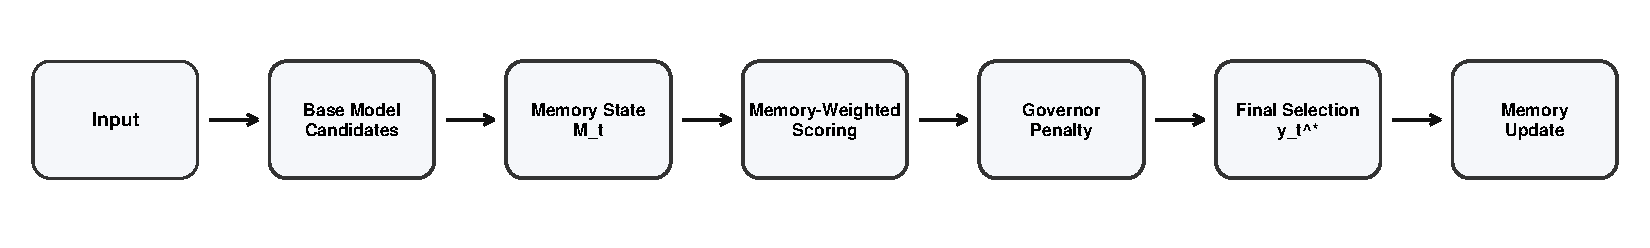
\includegraphics[width=\textwidth]{fig_architecture.pdf}
\caption{Reference architecture for memory-weighted candidate re-ranking.}
\label{fig:architecture}
\end{figure}

\section{Worked Scenarios}

The following examples are illustrative rather than empirical benchmark results. Their purpose is to show how the reference mechanism changes candidate selection relative to direct base-model emission.

\subsection{Continuity Across Prior Commitments}

Suppose a user has repeatedly indicated a preference for concise technical responses. A direct base-model emission may select a verbose explanation because it is broadly plausible for the input. Under memory-weighted selection, candidates aligned with the persistent preference receive higher memory scores, making a concise technical response more likely to be selected.

\subsection{Salience-Weighted Project Continuity}

Suppose an agent is assisting with a long-running software project in which prior interactions established a commitment to maintaining compatibility with an existing framework version. A generic candidate may recommend replacing major components with incompatible alternatives. A memory-weighted selection layer can penalise candidates inconsistent with persistent project constraints and favour candidates aligned with the established continuity requirements.

\subsection{Governor-Constrained Selection}

Suppose a user asks for guidance on a topic where prior interactions established a specific project preference. Candidate A is direct but inconsistent with prior commitments. Candidate B is moderately phrased but aligned with prior commitments and stability constraints. Candidate C is conservative but only weakly aligned.

Suppose three candidate outputs are produced for this input. Scores below are illustrative values on a normalized unit interval; practical implementations may use different scoring ranges depending on model architecture and calibration strategy.

\begin{table}[ht]
\centering
\begin{tabular}{lcccc}
\toprule
Candidate & Base Score & Memory Score & Governor Penalty & Final Score \\
\midrule
A & 0.82 & 0.18 & 0.35 & 0.44 \\
B & 0.74 & 0.32 & 0.05 & 0.92 \\
C & 0.69 & 0.22 & 0.02 & 0.84 \\
\bottomrule
\end{tabular}
\caption{Illustrative candidate scores under the reference objective.}
\label{tab:scenario}
\end{table}

Using illustrative weights:
\begin{equation}
\lambda_M = 0.8, \qquad \lambda_G = 1.5.
\end{equation}

Candidate B receives:
\begin{equation}
r(B,R_t)=0.32, \qquad \sigma(B,S_t)=0.41, \qquad a(B,A_t)=0.15,
\end{equation}
with component weights:
\begin{equation}
\alpha_R = 0.4, \qquad \alpha_S = 0.4, \qquad \alpha_A = 0.2.
\end{equation}
This gives:
\begin{equation}
s_{mem}(B \mid M_t)
=
(0.4 \times 0.32)
+
(0.4 \times 0.41)
+
(0.2 \times 0.15)
\approx 0.32.
\end{equation}

The final score for each candidate is computed as:
\begin{equation}
s_{final}(y)
=
s_{base}(y \mid x_t)
+
\lambda_M s_{mem}(y \mid M_t)
-
\lambda_G p_G(y).
\end{equation}

Candidate A receives the highest base-model score but incurs the largest governor penalty. Candidate B receives a lower base score but stronger alignment with the persistent memory state and a lower governor penalty. Under the reference selection objective, candidate B becomes the selected output.

This example is illustrative rather than empirical. Its purpose is to show how the reference formulation alters candidate ranking relative to direct base-model emission.

\begin{figure}[ht]
\centering
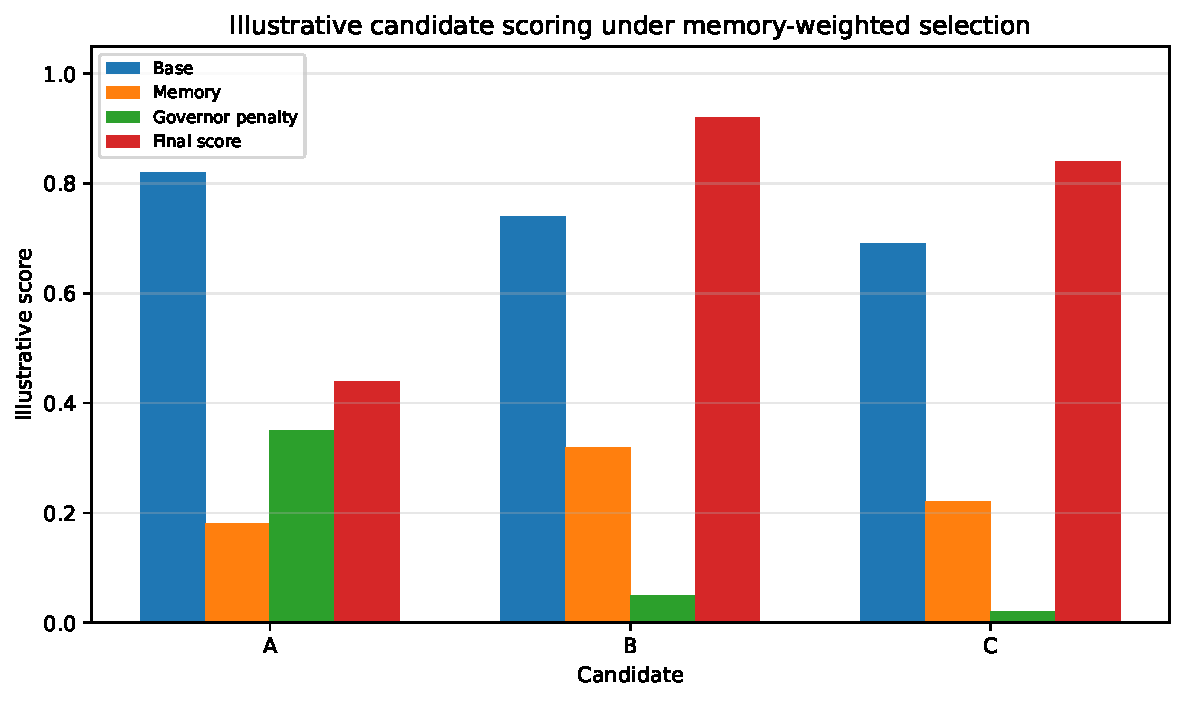
\includegraphics[width=0.85\textwidth]{fig_scenario.pdf}
\caption{Illustrative comparison of base score, memory score, governor penalty, and final score.}
\label{fig:scenario}
\end{figure}

\section{Reference Implementation Notes}

A prototype middleware instantiating the proposed architecture has been developed for internal evaluation. The present paper does not depend on production deployment claims. Instead, it describes the architectural principle and reference formulation that such a system can instantiate.

In a reference implementation, the base model or upstream generator produces multiple candidate outputs. The middleware receives these candidates, retrieves the current memory state, computes memory-alignment scores, applies governor penalties, and emits the selected candidate. After emission, the middleware records an update to the memory state, including recency metadata, salience indicators, and any anchor-relevant changes. In an applied software project, the same public structure may be described as governed, memory-weighted behavioural middleware: continuity memory, recency, salience, anchors, and WEL-style layered influence shape later candidate selection while private kernel logic and production thresholds remain undisclosed.

Production-specific parameterisations, internal scoring functions, governor policies, thresholds, persistence schemas, and kernel-level implementation details are outside the scope of this paper. The reference formulation is intended to be reproducible at the architectural level without disclosing proprietary implementation details.

\section{Limitations}

This paper presents a reference formulation and architecture, not a large-scale empirical evaluation. The worked scenarios are designed to clarify mechanism behaviour and do not constitute benchmark validation.

The formulation does not prescribe a single optimal memory-scoring function, governor policy, or parameter schedule. Different implementations may require different similarity functions, salience estimates, decay rates, and penalty functions.

The proposed architecture does not replace base models, retrieval systems, RLHF, constrained decoding, reranking systems, best-of-N selection, or moderation systems. It can be understood as a middleware-level selection mechanism that may be combined with those methods.

The paper makes no claim about consciousness, sentience, agency, cognition, physics, field-theoretic interpretation, quantum measurement, or artificial general intelligence. Its claim is limited to middleware-level candidate selection in LLM systems.

\section{Future Work}

Future work should focus on empirical evaluation on continuity and governance benchmarks; comparison against baseline memory architectures, retrieval-augmented systems, conventional rerankers, and direct base-model emission; characterisation of parameter sensitivity for $\lambda_M$, $\lambda_G$, and component weights $\alpha_R$, $\alpha_S$, $\alpha_A$; and extensions to multi-agent and longer-horizon settings.

\bibliographystyle{plainnat}
\bibliography{references}

\end{document}
